\chapter{Case Study: Diffraction through the Pinhole}

% MENTION THE CUTOFF OF THE GAUSSIAN FILTER (optional)
% HDR - VP - 2? Not needed now
% Don't forget to rerun the 25 micron pinhole mask

One important question to ask about the vision correcting display is: "What is the optimal pinhole size for the pinhole mask?" The regular simulation applies ray optics, which does not take into account properties of light, such as diffraction and interference. We want a new simulation that models the effects of diffraction through a pinhole.

\section{Software Simulation - Wave Optics}

We utilize another approach to the software simulation that considers both light traveling as a ray and the diffraction effects of the pinhole. 

\subsection{Fraunhofer Diffraction through Rectangular Aperture}
\noindent We assume that a light source emits a spherical wavefront that creates a constant electric field on the pinhole. We consider each screen pixel as a point source, and since the depth of the pinhole mask (6 millimeters) is much larger than the size of the screen pixel (78 micrometers) or the pinhole (75 micrometers), the value of the electric field will not vary significantly between the edges of the pinhole and center of the pinhole. The distance between the pinhole plane and the sensor plane is about 27 centimeters, which is much larger than the size of the sensor, so there is not a large variation in the length of different light rays traveling from the mask to the sensor. The pinholes are squares, and we meet the conditions for Fraunhofer diffraction through a rectangular aperture \cite{Lipson:1987:OpticalPhysics}: 
$$\frac{W^2}{L \times \lambda} \ll 1$$
Here, $W$ is the length of the aperture, $L$ is the distance of the sensor from the aperture, and $\lambda$ is the wavelength. $W$ is at most $125$ micrometers, $L$ is roughly $27$ centimeters, and $\lambda$ is about $500$ nanometers. 

\begin{figure}[ht]
  \centering
  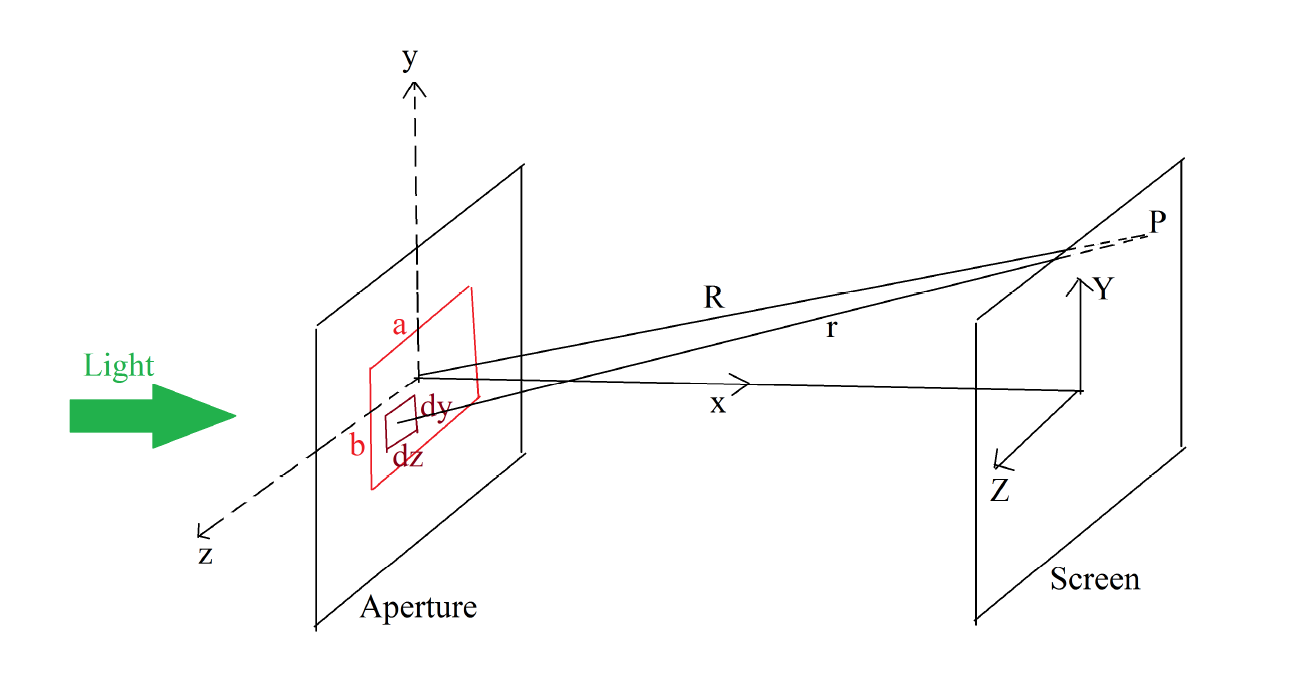
\includegraphics[width=4in]{chapters/chapter8/images/Rectangular_Aperture.png}
  \caption{Fraunhofer Diffraction through Rectangular Aperture Diagram \cite{Rao:2014:FraunhoferDiffraction}}
  \label{fig:rectangle_aperture}
\end{figure}

Let $\epsilon_A$ represent the electric field strength per unit area, which is assumed to be constant over the entire aperture (derivation below from Hecht 1987 \cite{Hecht:1987:Optics}). The electric field contributed by the small section of the aperture $dzdy$ at point P on the screen is 
$$dE = \left(\frac{\epsilon_A}{R} \right)e^{i(\omega t-kr)}dzdy$$
where $r = [X^2 + (Y-y)^2+(Z-z)^2]^{\frac{1}{2}}$ and $k = \frac{2 \pi}{\lambda}$, the wavenumber. We can use the far field approximation and set $r = R$ for the amplitude term and $r = R[1-(Yy+Zz)^2/{R^2}]$ in the phase term. The total electric field at point $P$ on the screen is \\
$$E = \left(\frac{\epsilon_{A}}{R}\right)e^{i(\omega t-kR)} \int_{-b/2}^{b/2} e^{ikYy/R}dy \int_{-a/2}^{a/2} e^{ikZz/R} dz $$
Solving the integral gives \\
$$E = \left(\frac{ab\epsilon_A}{R}\right) e^{i(\omega t-kR)} sinc\left(\frac{kaZ}{2R}\right)sinc\left(\frac{kbY}{2R}\right) $$ \\
Intensity is equal to the square of the amplitude of the electric field intensity, so \\
$$I(Y,Z) = Re\left[\left(\frac{ab\epsilon_A}{R}\right)e^{i(\omega t - kR)} sinc\left(\frac{kaZ}{2R}\right) sinc\left(\frac{kbY}{2R}\right)\right]^2$$
$$I(Y,Z) = I_0  sinc^2\left(\frac{kaZ}{2R}\right) sinc^2\left(\frac{kbY}{2R}\right)$$
Intensity of light is proportional to two $sinc$ squared functions multiplied in both the $Y$ and $Z$ directions.
% In the future, try to justify your new model.


\subsection{Diffraction through a Lens}
The above diffraction equation creates a very large diffraction pattern on the sensor that leads to far too much loss of contrast. To fix this,we need to consider the effects of the lens and the fact that the display is not placed at the focus distance of 380 millimeters. 

\begin{figure}[ht]
  \centering
  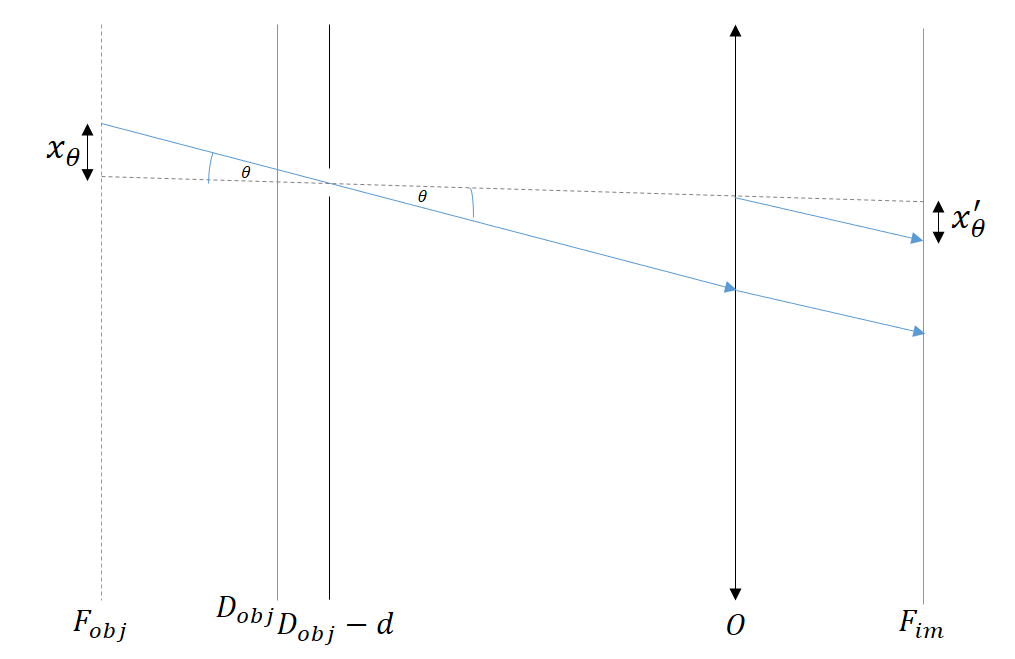
\includegraphics[width=4in]{chapters/chapter8/images/Lens_Diffraction.png}
  \caption{Fraunhofer diffraction through lens. $F_{obj}$ is the focus distance, $D_{obj}$ is the display distance, $d$ is the depth of the pinhole mask, $O$ is the plane of the lens, and $F_{im}$ is equal to position of the sensor at focus.}
  \label{fig:ferrari}
\end{figure}

We know that $$I(Y,Z) = I_0  sinc^2\left(\frac{kaZ}{2R}\right) sinc^2\left(\frac{kbY}{2R}\right)$$
We substitute in $sin(\theta) \sim \frac{Z}{R}$ and $sin(\phi) \sim \frac{Y}{R}$:
$$I(\theta,\phi) = I_0  sinc^2\left(\frac{\pi a sin \theta}{\lambda}\right) sinc^2 \left(\frac{\pi b sin \phi}{\lambda}\right)$$

We want to find the shape of the diffraction pattern as a function of sensor coordinates, $x_{\theta}'$ and $x_{\phi}'$. In other words, we want to determine $I(x_{\theta}', x_{\phi}')$, where $x_{\theta}'$ is the image created by $x_{\theta}$ and $x_{\phi}'$ is the image created by $x_{\phi}$. 

We consider the angle that light travels through the pinhole, and imagine that the light ray is traced back to the plane at the focus distance. We have: 
$$tan(\theta) = \frac{x_{\theta}}{F_{obj} - D_{obj} + d}$$ 
which gets rearranged to 
$$x_{\theta} = (F_{obj} - D_{obj} + d) tan\theta$$

Then, based on the displacement $x_{\theta}$ on the focus object plane, we can compute the displacement on the sensor $x_{\theta}'$ through the magnification equation. 

$$x_{\theta}' = x_{\theta} \frac{F_{im}}{F_{obj}} =  \frac{F_{im}}{F_{obj}} (F_{obj} - D_{obj} + d) tan\theta $$

Likewise, $$x_{\phi}' = x_{\phi} \frac{F_{im}}{F_{obj}} =  \frac{F_{im}}{F_{obj}} (F_{obj} - D_{obj} + d) tan\phi $$

We want to incorporate the expressions for $x_{\theta}'$ and $x_{\phi}'$ into the original intensity equation. We use the conditions $\theta \ll 1$ (and $\phi \ll 1$) to make the approximations $sin\theta \approx tan\theta \approx \theta$ and $sin\phi \approx tan\phi \approx \phi$. Therefore, 

$$I(\theta, \phi) \approx I_0 sinc^2\left(\frac{\pi a \theta}{\lambda}) sinc^2(\frac{\pi b \phi}{\lambda}\right)$$

We rearrange $$x_{\theta}' = \frac{F_{im}}{F_{obj}} (F_{obj} - D_{obj} + d) \theta $$ to get $$\theta =  \frac{F_{obj}} {(F_{obj} - D_{obj} + d)F_{im}} x_{\theta}'$$ Likewise,  $$\phi =  \frac{F_{obj}} {(F_{obj} - D_{obj} + d)F_{im}} x_{\phi}'$$ We substitute these results into the intensity equation to get

$$I(x_{\theta}', x_{\phi}') \approx $$ $$I_0 sinc^2 \left(\frac{\pi a F_{obj} x_{\theta}'}{F_{im}(F_{obj} - D_{obj} + d)\lambda}\right) sinc^2 \left(\frac{\pi b F_{obj} x_{\phi}'}{F_{im}(F_{obj} - D_{obj} + d)\lambda}\right)$$

\subsection{Integration of Ray and Wave Optics}

In the integrated ray and wave optics model, ray optics determines the direction of light rays, and wave optics determines the size of the diffraction pattern on the sensor. We continue to do backwards ray tracing on multiple aperture samples, but each ray creates a diffraction pattern on multiple sensor pixels. The combined model is equivalent to blurring the result of the ray optics image by applying a low pass filter, and the blur matrix is a 2D array of intensities from the Gaussian diffraction pattern. We apply a different blur matrix for each color because different colors have different wavelengths and therefore diffraction patterns of varied sizes.

\begin{figure}[ht]
  \centering
  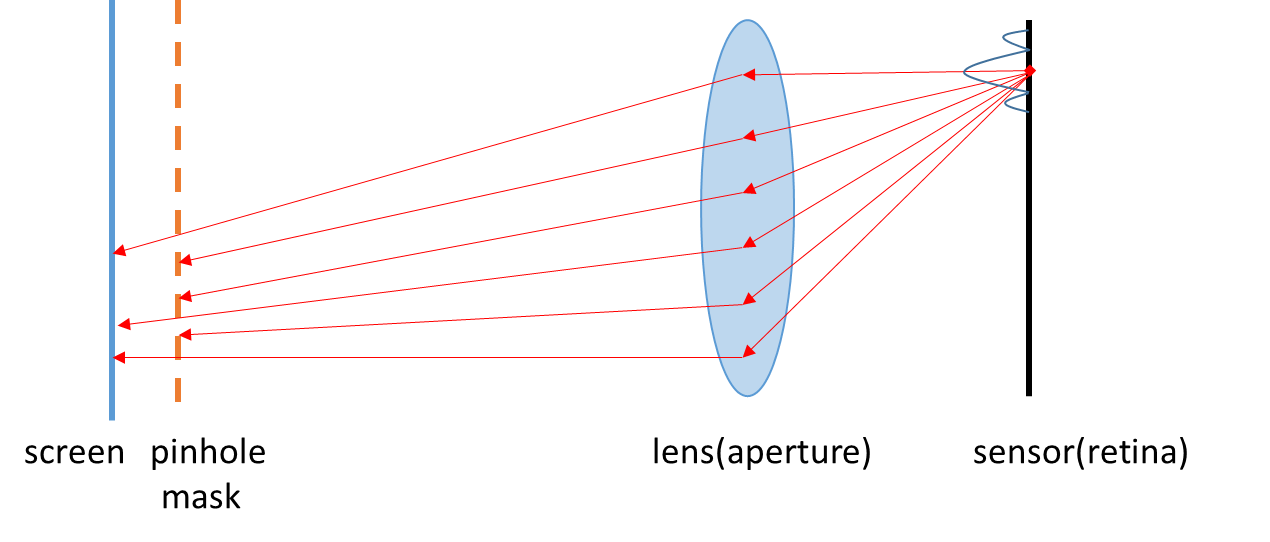
\includegraphics[width=4in]{chapters/chapter8/images/Diffract_Simulation.png}
  \caption{Wave Optics Simulation}
  \label{fig:ferrari}
\end{figure}


\begin{lstlisting}[frame=single, basicstyle=\footnotesize\ttfamily, caption=Pseudocode For Wave Optics Simulation]
int[][][] sensor = new int[sensor_size][sensor_size][3];
// Iterate over sensor pixels
for (int iy = 0; iy < sensor_size; iy++) {
  for (int ix = 0; ix < sensor_size; ix++) {
    int color[3] = {0, 0, 0};
    int hits = 0;
    // Iterate through random aperture points
    for (int i = 0; i < aperture_sample_time; i++) {
      sensor_pos = (ix, iy);
      aperture_pos = (aperture_samples[2*i], aperture_samples[2*i + 1]);
      type,color = getRayColor(sensor_pos, aperture_pos);
      if (value >= 0) {
        hits++;
	color[type] += value;
      }
    }
  }
  for (int x = 0; x < diffractMatrix.length; x++) {
    for (int y = 0; y < diffractMatrix.width; y++) {
       sensor[ix + x - diffractMatrix.length / 2][iy + y - 
       diffractMatrix.width/2] += intensity[x][y] * color * 3 / hits;
    }
  }
}
\end{lstlisting}

\section{Results}

We compare the images produced by the physical experiment, ray optics simulation, and wave optics simulation. The parameters for all three cases are the same as those described earlier in the physical experiment section (380 millimeters focus distance, 250 millimeters display distance, 6 millimeters depth of pinhole mask, 6 millimeters diameter of human eye or f/8 stop, and 20 millimeters focal length). In addition, to see how well the ray and wave optics model account for diffraction, we examine the image quality of multiple pinhole sizes.

\subsection{Metrics}

The two metrics used to measure image quality are DRIM (dynamic range imagery) and RMSE (root mean square error).

\subsubsection{DRIM}

Aydin et. al 2008 \cite{aydin2008dynamic} describes DRIM as a metric that enables comparison of images with different dynamic ranges. The paper describes three measurements of image distortion: loss of visible contrast, amplification of invisible contrast, and reversal of visible contrast. We focus on loss of visible contrast, which occurs when contrast that was visible in the reference image becomes invisible in the test image. The algorithm in the paper applies a loss of visible contrast predictor and then a high-pass or low-pass filter. Figure 8.4 shows the distortion maps for the wave optics model for a 75 micrometer pinhole:

\begin{figure}[ht]
  \centering
  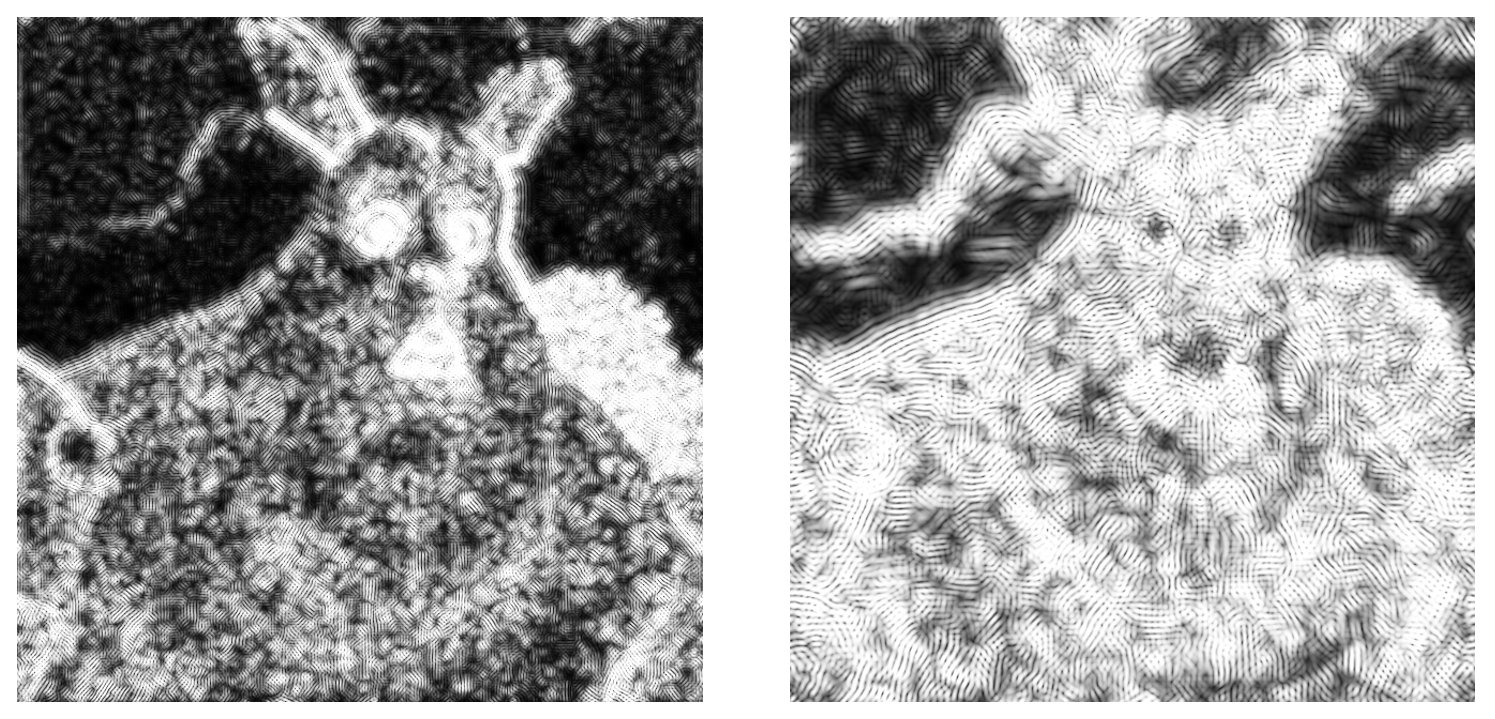
\includegraphics[width=3.5in]{chapters/chapter8/images/hp_lp_contrast_loss.png}
  \caption{Contrast Loss High Pass (left) and Contrast Loss Low Pass (right)}
  \label{fig:ferrari}
\end{figure}

The bright pixels represent areas of contrast loss. We compute the contrast loss as the pixel sum of the low-pass distortion image plus the pixel sum of the high-pass distortion image divided by two. 

\subsubsection{RMSE}

RMSE is a measurement used to measure how close the pixel values of the test image are to the reference image. $I_r$ in the equation below represents the RGB (red, green, and blue) intensities of the reference image, and $I_t$ represents the RGB intensities of the simulated image.

$$RMSE = \sqrt{ \sum_{y = 0}^{\textnormal{image length}} \sum_{x = 0}^{\textnormal{image width}} \sum_{c \in \{r,g,b\}} (I_r (x,y,c) - I_s(x,y,c))^2}$$

\subsection{Comparison of Ray and Wave Optics}

\begin{figure}[ht]
  \centering
  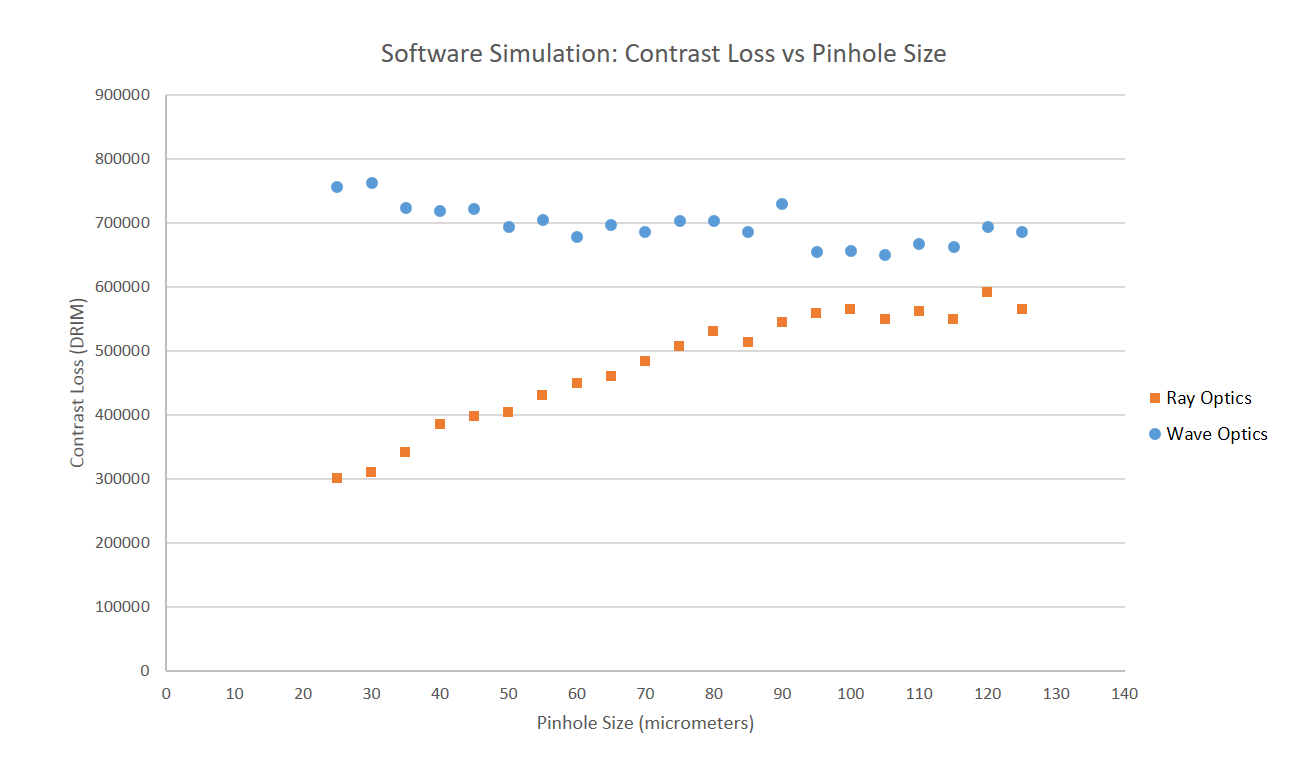
\includegraphics[width=7.0in]{chapters/chapter8/images/Contrast_Loss.png}
  \caption{DRIM Graph}
  \label{fig:ferrari}
\end{figure}

For the ray optics model, the larger the pinhole size, the worse the contrast. The pinhole size that gives the least loss of contrast is 25 micrometers. A pinhole of size 120 micrometers (contrast loss of about 600,000) generates twice the amount of contrast loss as a pinhole of size 25 micrometers (contrast loss of about 300,000). These results are expected because smaller pinholes block more light rays, which leads to sharper image contrast. For the combined ray and wave optics model, the contrast loss from different-sized pinholes is roughly the same (between 640,000 and 770,000). We find that the benefits of a small aperture in filtering light are counterbalanced by the larger diffraction pattern that is created. The smallest pinhole sizes create the largest diffraction patterns and therefore have the most severe contrast loss. From 25 micrometers to 105 micrometers, there is a weak trend of improving contrast due to the effects of diffraction outweighing the sharper focus of light through the pinhole. From 105 micrometers to 125 micrometers, there is a weak trend of declining contrast because at that point, the diffraction effects are very minor, and the larger pinhole sizes reduce the depth of field and do not focus the light source well. A pinhole size of 105 microns generates an image with the most contrast.

\begin{figure}[ht]
  \centering
  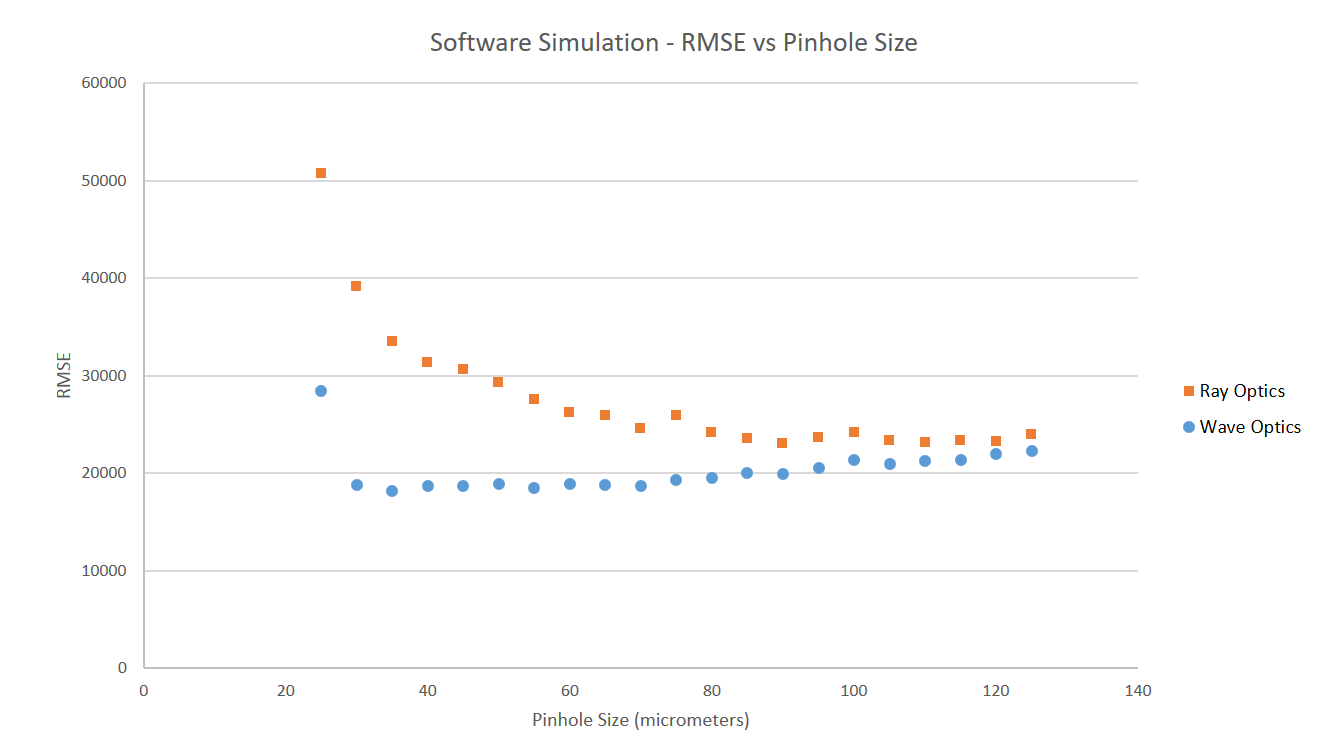
\includegraphics[width=7.0in]{chapters/chapter8/images/RMSE.png}
  \caption{RMSE Graph}
  \label{fig:ferrari}
\end{figure}

For the RMSE metric, the wave optics model features improvement over the ray optics model, despite the fact that the wave optics model produces a blurred version of the ray optics model. For both models, small pinhole sizes create an amplification of contrast, which leads to a larger RMSE. In addition, since small pinhole sizes allow significantly fewer light rays to reach the screen, there is a greater possibility of having too many rays of one color (red, green, or blue) and getting a noisy image (see figure 14 below). Because blurring reduces this amplification of contrast, larger pinhole sizes have smaller RMSE values for the ray optics model, and the wave optics model consistently produces images with smaller RMSE than the ray optics model. The wave optics model shows a trend of increasing RMSE for pinhole sizes 75 micrometers and above, because at that point, there is no more amplification of contrast, and blurring only causes the modeled image to deviate further from the clean image. Although a smaller RMSE is expected to indicate a image with pixel values close to the original image, it actually has a high chance of indicating more blur. Therefore, RMSE is a poor indicator of contrast and mediocre indicator of image quality. 

\begin{figure}[ht]
  \centering
  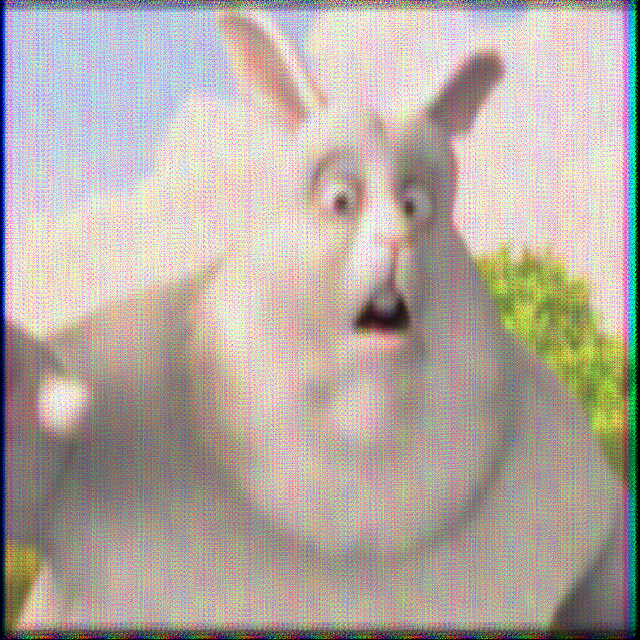
\includegraphics[width=2in]{chapters/chapter8/images/simulationResult_25.png}
  \caption{Ray Optics Simulation for 25 micrometer pinhole mask}
  \label{fig:ferrari}
\end{figure}

\subsection{Comparison of Physical Experiment and Software Simulation}

\begin{figure}[ht]
  \centering
  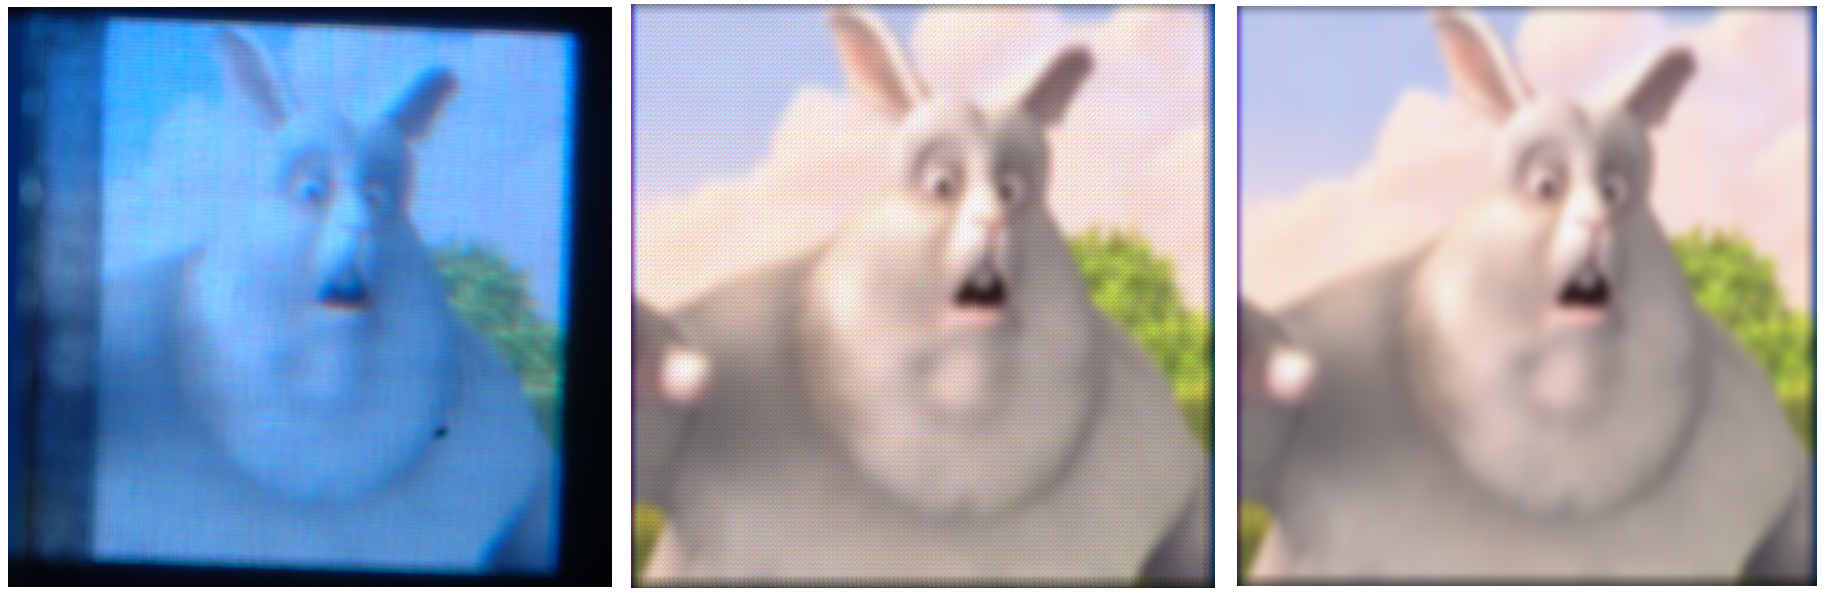
\includegraphics[width=6in]{chapters/chapter8/images/Comparison.png}
  \caption{Left: Physical Experiment, Center: Ray Optics Simulation, Right: Wave Optics Simulation}
  \label{fig:ferrari}
\end{figure}
% TODO: Need a zoomed in version of each picture

\begin{figure}[ht]
  \centering
  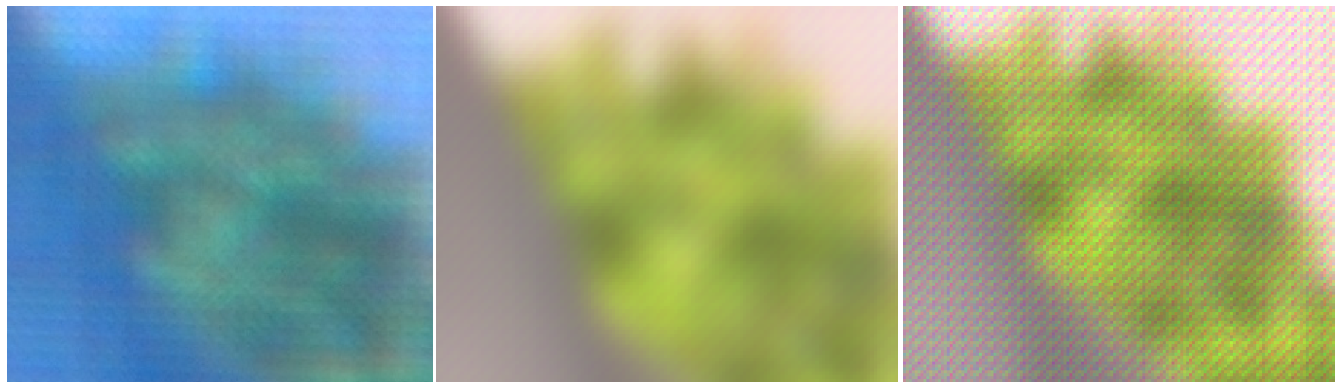
\includegraphics[width=6in]{chapters/chapter8/images/comparison_zoom.png}
  \caption{Zoomed Version of Pictures }
  \label{fig:ferrari}
\end{figure}

We compare the images produced by the physical experiment, ray optics simulation, and wave optics simulation for a 75 micrometer pinhole. The wave optics simulation is slightly more blurred than the ray optics simulation, which is expected. Interestingly enough, the physical simulation generates the clearest image, but the exposure had to be inflated in order for the physical simulation to work. If one looks closely at the physical experiment image and the ray simulation image, one will find that a grid pattern is visible on the physical experiment image and especially the ray optics image, but is removed from the wave optics image due to diffractional blur. This shows that perhaps the wave optics simulation created a blur pattern that was too large for the 75 micrometer pinhole. 

\section{Conclusion and Future Work}

The physical experiment and the software simulation give mixed results. The prefiltering algorithm combined with the pinhole mask display yields a significant improvement to the defocused image. The ray optics model yields an image that has slightly less contrast than the one in the physical experiment and recommends using the smallest pinhole size to achieve the best contrast as long as RMSE is not too high. The wave optics model gives even more blurred images than the ray optics model and recommends using a larger pinhole size of approximately 105 micrometers to achieve an image with the best contrast. There exists a slight contrast gap between the physical experiment and software simulations that needs to be resolved.

In the future, we will try to find more ways to improve on the ray and wave optics model to look more like the physical experiment. One area to expand on in the wave optics model is to consider the light ray as a Gaussian beam rather than a point source. In addition, we would like to test the ray and wave optics models for astigmatism, another form of lower order aberrations, and higher order aberrations like coma and trefoil. We would also be interested in running physical experiments with pinhole masks for different sizes to confirm the results of the ray and wave optics models. 